\documentclass{beamer}

\usepackage{tikz}
\usepackage[percent]{overpic}
\usetikzlibrary{calc,trees,positioning,arrows,fit,shapes,calc}
\usepackage{verbatim}
\usepackage{stmaryrd}
\usepackage{amsmath}
\usepackage{amssymb}

\usepackage{color}
\usepackage[percent]{overpic}

\definecolor{fgreen}{RGB}{34,139,34}

\usetheme{Berlin}
\title{A New Approach to Sample Deconvolution}
\author{Greg Hunt}
\institute{University of Michigan}
\date{December 9, 2016}


\beamertemplatenavigationsymbolsempty
\addtobeamertemplate{navigation symbols}{}{%
    \usebeamerfont{footline}%
    %\usebeamercolor[fg]{footline}%
    \color{black}
    \large
    \hspace{1em}%
    \insertframenumber/\inserttotalframenumber
}

\usepackage{remreset}% tiny package containing just the \@removefromreset command
\makeatletter
\@removefromreset{subsection}{section}
\makeatother
\setcounter{subsection}{0}

\begin{document}

\section{Introduction}
\subsection{}

\begin{frame}
\titlepage
\end{frame}

\begin{frame}
  \frametitle{Deconvolution = Decomposing Mixtures}
  \begin{center}
    {\color{blue}Convolution: $X,Y \rightarrow X+Y$, \quad Deconvolution $X+Y \rightarrow X,Y$}
  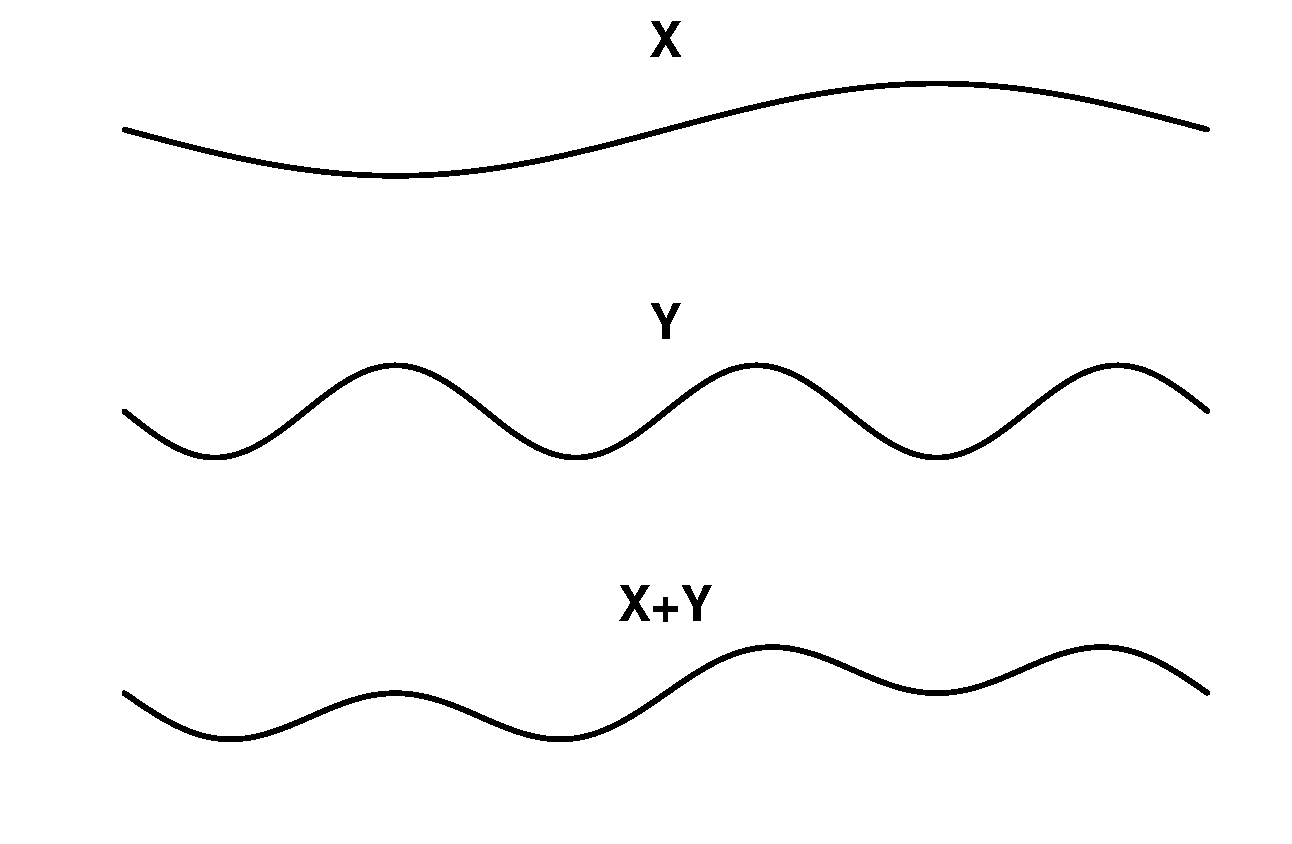
\includegraphics[scale=.4]{sigconv.pdf}
  \end{center}
\end{frame}

\begin{frame}
  \frametitle{Sample Deconvolution = Decomposing Expression Data}
  \begin{center}
    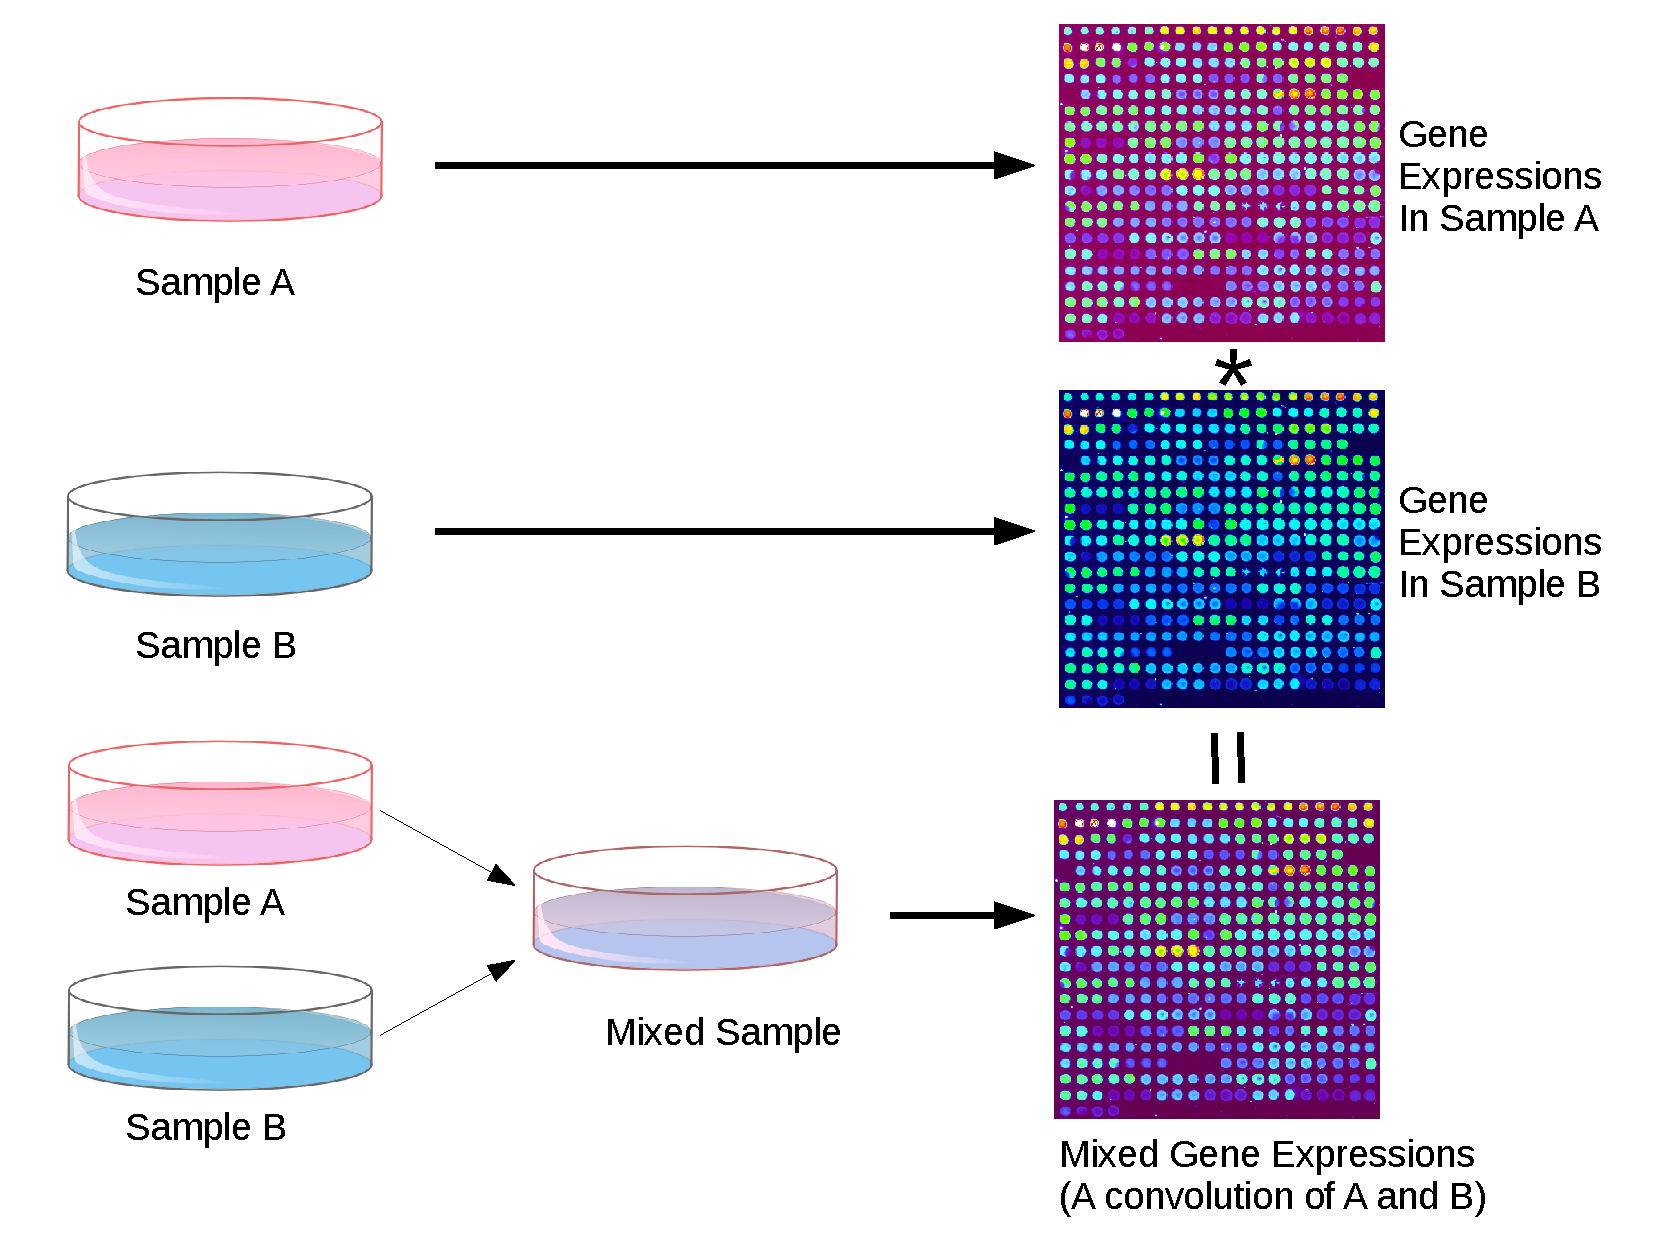
\includegraphics[scale=.3]{slide_conv.pdf}
      {\tiny Image Credits: [1,2]}
  \end{center}
\end{frame}

\setcounter{subsection}{0}
\section{Scientific Background}
\subsection{}

\begin{frame}
  \frametitle{}
  \begin{center}
  {\color{blue}{\Huge
      Scientific Background
  }}
  \end{center}
\end{frame}


\begin{frame}
  \frametitle{Measure Gene Expression by Counting mRNA}
  \begin{columns}
    \begin{column}{0.48\textwidth}
      \begin{center}
        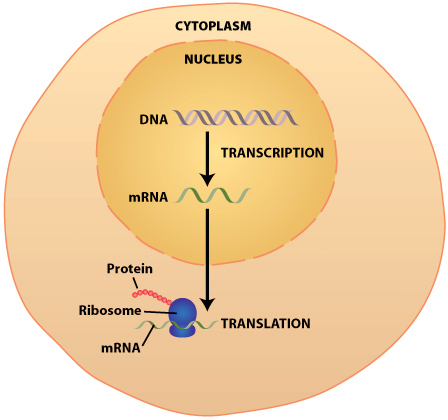
\includegraphics[scale=.35]{ribo.jpg}
      \end{center}
    \end{column}
    \begin{column}{0.48\textwidth}
      Every time a gene is expressed an mRNA specific to that gene is created. 
    \end{column}
  \end{columns}
      {\tiny Image Credits: [4]}
\end{frame}

\begin{frame}
  \frametitle{Microarrays Determine which Oligos are Present}
  \begin{columns}
    \begin{column}{0.48\textwidth}
      \begin{enumerate}
      \item[(1)] Extract mRNA chunks ({\color{blue} oligonucleotides} or {\color{blue}oligos}).
      \end{enumerate}
      \begin{center}
        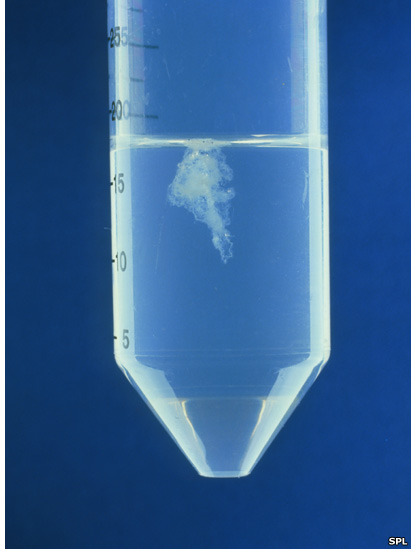
\includegraphics[scale=.2]{extracteddna.jpg}
      \end{center}
    \end{column}
    \begin{column}{0.48\textwidth}
      \begin{enumerate}
        \item[(2)] Determine which oligos present with microarray. 
      \end{enumerate}
      \begin{center}
        \includegraphics[scale=.55]{mascale.png}
      \end{center}
    \end{column}
  \end{columns}

  {\tiny Image Credits: [5,6]}
  
\end{frame}

\begin{frame}
  \frametitle{Microarrays are a Collection of Probes}
  \begin{columns}
    \begin{column}{0.48\textwidth}
      \begin{center}
        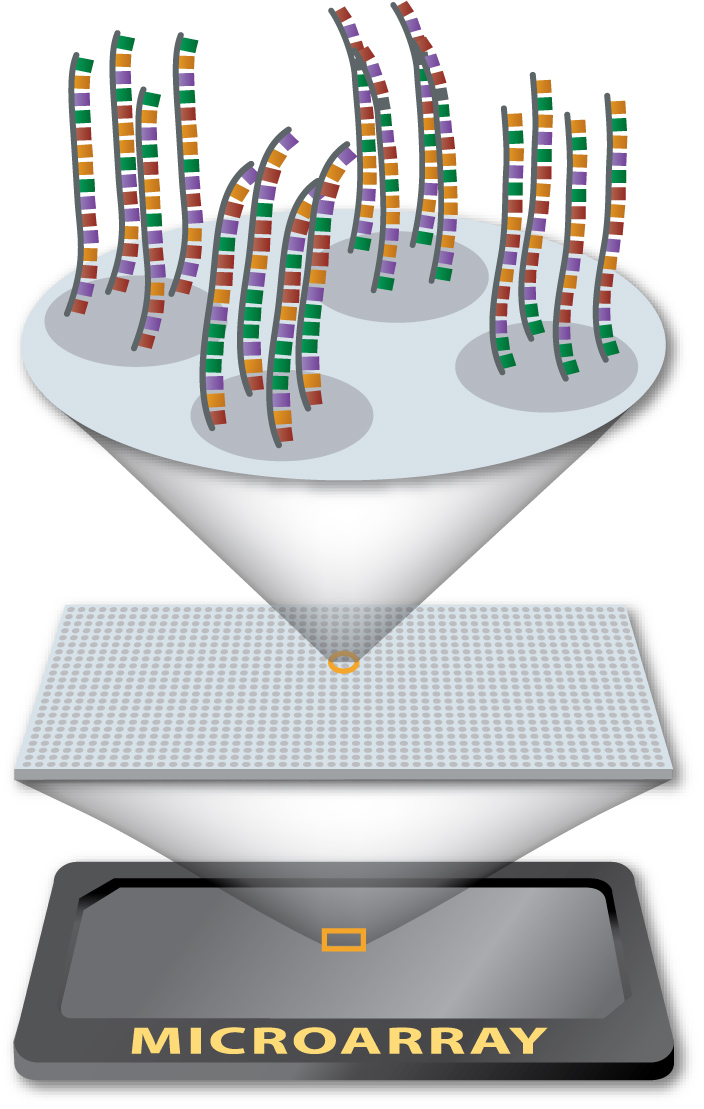
\includegraphics[scale=.15]{mazoom.jpg}
      \end{center}
    \end{column}
    \begin{column}{0.48\textwidth}
        Probe spots on microarray each tell about abundance of a different oligo.

    \end{column}
  \end{columns}

  {\tiny Image Credits: [7]}
\end{frame}

\begin{frame}
  \frametitle{Fluorescence of a Probe = Abundance of an Oligo}
  \begin{columns}
    \begin{column}{0.48\textwidth}
      \begin{center}
        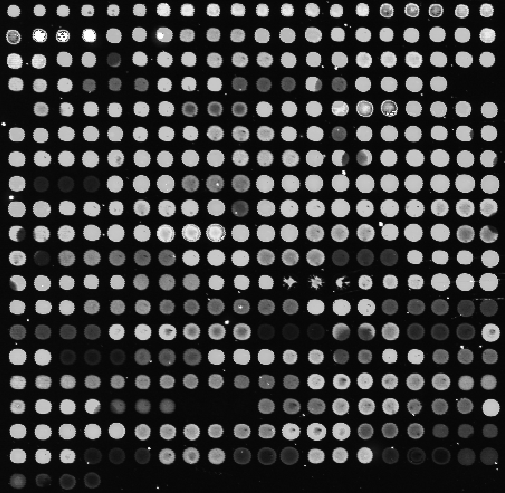
\includegraphics[scale=.4]{fluor_bw.png}
      \end{center}
    \end{column}
    \begin{column}{0.48\textwidth}
      Fluorescence of each probe tells us how much of that type of oligo is present. 
    \end{column}
  \end{columns}
\end{frame}

\begin{frame}
\frametitle{Microarray Data is Probe Intensities}
Microarray data is intensity measurements $I_1,\ldots,I_{\color{blue}N}$\vspace{.1cm}

Typically {\color{blue}$N\approx 500,000$}


{\small \begin{center}
    {\bf Example:}
    \begin{tabular}{c||c|c|c|c|c}
      Probe Name& 1367452\_at& 1367453\_at& 1367454\_at& 1367455\_at& $\cdots$\\\hline
      Intensity& 84&       5063&        140&       5065&        $\cdots$
    \end{tabular}
  \end{center}}

  A common data pre-processing step is to {\color{blue}logarithmically} tranform.

  {\small \begin{center}
          {\bf Example:}
    \begin{tabular}{c||c|c|c|c|c}
      Probe Name& 1367452\_at& 1367453\_at& 1367454\_at& 1367455\_at& $\cdots$\\\hline
      log(Intensity)& 6.39&       12.305&       7.129&       12.306&        $\cdots$
    \end{tabular}
  \end{center}}
\end{frame}

\setcounter{subsection}{0}
\section{Literature}
\subsection{}

\begin{frame}
  \frametitle{}
  \begin{center}
  {\color{blue}{\Huge
    Literature Review
  }}
  \end{center}
\end{frame}

\begin{frame}
  \frametitle{The Common Model is Linear}
  Consider {\color{blue}$S$} samples
  \begin{enumerate}
  \item Each sample mixture of {\color{blue}$K$} cell types.
  \item Measurements of {\color{blue}$N$} oligos in each sample. 
  \end{enumerate}

  \vspace{.25cm}
  The Model:
  \[
  \underbrace{\begin{bmatrix}
    \quad& & \quad\\
    \quad& \text{{\Huge X}}_{S\times N}& \\
    \quad& & \quad
    \end{bmatrix}}_{
      \text{data matrix}
  }
  =
    \underbrace{\begin{bmatrix}
    \quad& & \quad\\
    \quad& \text{{\Huge M}}_{S\times K}& \\
    \quad& & \quad
    \end{bmatrix}}_{
      \text{mixing matrix}
  }
  \underbrace{\begin{bmatrix}
    \quad& & \quad\\
    \quad& \text{{\Huge U}}_{K\times N}& \\
    \quad& & \quad
    \end{bmatrix}}_{
      \text{characteristic expressions}
  }
  +
  E
  \]
  for error matrix $E$.
  %\begin{enumerate}
  %\item Data matrix $X\in\mathbb{R}^{S \times N}$ where $X_{sn}$ is $n^{th}$ oligo expression in $s^{th}$ sample
  %\item Mixing matrix $M \in\mathbb{R}^{S \times K}$ where $M_{sk}$ is percent of $s^{th}$ sample that is type $k$
  %\item Characteristic expression profiles $U \in\mathbb{R}^{K \times N}$ so that $U_{kn}$ is typical expression of $n^{th}$ oligo in type $k$
  %\end{enumerate}
\end{frame}

\begin{frame}
  \frametitle{Our Goal: Predict the Mixing Proportions}
  We always know $X$ and model it as
  \[
  X = MU+E
  \]
  We may not know $U$ or $M$.\newline
  
Two types of deconvolution:\newline
  {\color{blue}{\bf Partial Deconvolution}}
  \begin{enumerate}
  \item[1] Know $U$ and predict $M$
  \item[2] Know $M$ and predict $U$
  \end{enumerate}
  
  {\color{blue}{\bf Full Deconvolution}}
  \begin{enumerate}
  \item[3] Know neither $M$ nor $U$ and predict jointly
  \end{enumerate}

  \begin{center}
    {\Large {\color{blue}We are interested in (1): predicting $M$ given $U$.}}
    \end{center}

\end{frame}

\begin{frame}
  \frametitle{Literature: Similar Model, Different Fitting}
  \begin{block}{Problem}
    Assume known $X$, $U$,
    \[
    X = MU + E
    \]
    and solve for $M$.

    {\bf Constraint:} $M$ must be a row-wise probability matrix. 
  \end{block}

  {\bf Solutions:}
  \begin{enumerate}
  \item {\color{blue}Regression}: regress $X$ on $U$ so that elements of $M$ are regression coefficients. Somehow enforce constraints.
  \item {\color{blue}Bayesian}: Similar to LDA. Estimate as MAP. 
  \end{enumerate}

  \begin{center}
    {\Large {\bf Idea:} {\color{blue} marker oligos}.}
    \end{center}
\end{frame}

\begin{frame}
  \frametitle{Marker Oligos are Oligos Expressed in Only One Cell Type}

  {\color{blue}Empirically models have better fit if restricted to marker oligos.\newline}

  {\bf Idea:} Find marker oligos for each cell type. Restrict analyis to marker oligos only.
    \begin{enumerate}
    \item Can be as simple as fitting using submatrices.
    \item Many different ways to select markers. Usually chosen by looking at {\color{blue} pure samples}. 
    \end{enumerate}
\end{frame}

\begin{frame}
  \frametitle{Pure Samples are Training Data}
  Most methods require a pure sample of each of the $K$ cell types. 

  \begin{enumerate}
    \item Used to find markers.
    \item Can give us $U$.
    \end{enumerate}
\end{frame}

\begin{frame}
  \frametitle{Other Minor Variations in the Literature}
  Model:
  \[
  X = MU+E
  \]
  
  Ways to solve this partial deconvolution problem differ by
  \begin{enumerate}
  \item Fitting methods.
  \item Marker oligo choices.
  \item Construction of $U$
  \item {\color{blue}{\bf Transformations:}} e.g. do a logarithmic transformation.
  \item {\color{blue}{\bf Summarizations:}} summarize probes into genes using RMA or MAS5. 
  \end{enumerate}
  
\end{frame}

\setcounter{subsection}{0}
\section{Our Method}
\subsection{}

\begin{frame}
  \frametitle{}
  \begin{center}
  {\color{blue}{\Huge
      New Methodology
  }}
  \end{center}
\end{frame}


\begin{frame}
  \frametitle{Toy Example: Two Cell Types}

  Assume we have {\color{blue} two cell types} and three samples.
  \begin{enumerate}
  \item {\color{blue}$A$} = pure sample of type one.
  \item {\color{blue}$B$} = pure sample of type two.
  \item {\color{blue}$C$} = mixture sample.
  \end{enumerate}\vspace{.25cm}

Define:
{\Large  \[
\eta_{{\color{blue}A}{\color{red}n}} = \text{concentration of oligo {\color{red}n} in sample {\color{blue}$A$}}
\]}

Similarly for $\eta_{{\color{blue}B}{\color{red}n}}$ and $\eta_{{\color{blue}C}{\color{red}n}}$.
\end{frame}

\begin{frame}
  \frametitle{Our Concentration/Expression Model is Linear}
  {\Large {\color{blue}$Y_{An}$} $=$ $\log_2$(expression of oligo $n$ in sample $A$.)}\newline

  Similarly define {\color{blue}$Y_{Bn}$} and {\color{blue}$Y_{Cn}$}.\vspace{.25cm}

  Assume the linear relationship between {\color{red} concentration} and {\color{blue} expression}
  \[
  \begin{aligned}
    {\color{blue} Y_{An}} &= \theta_n + \gamma\log_2\left({\color{red}\eta_{An}}\right)+\epsilon_{An}\\
    {\color{blue} Y_{Bn}} &= \theta_n + \gamma\log_2\left({\color{red}\eta_{Bn}}\right)+\epsilon_{Bn}\\
    {\color{blue} Y_{Cn}} &= \theta_n + \gamma\log_2\left({\color{red}\eta_{Cn}}\right)+\epsilon_{Cn}
  \end{aligned}
  \]
  for all $n=1,\ldots,N$. Where the $\epsilon$ are i.i.d with mean zero and constant variance. 
\end{frame}
\begin{frame}
  \frametitle{Truth is Non-Linear but Linear Model is Reasonable}
  Remember the linear model: {\color{blue}$Y_n = \theta_n+\gamma\log_2\left(\eta_n\right)+\epsilon$}
  \begin{figure}
    \begin{overpic}[width=0.5\textwidth,tics=10]{plot1}
      \put (-10,50) {\color{blue} \large$Y_n$}
      \put (50,-5) {\color{blue} \large$\log_2\eta_n$}
\end{overpic}
    \caption{Relationship between concentration and expression.}
  \end{figure}
\end{frame}

\begin{frame}
  Remember the linear model: {\color{blue}$Y_n = \theta_n+\gamma\log_2\left(\eta_n\right)+\epsilon$}
    \frametitle{Truth is Non-Linear but Linear Model is Reasonable}
  \begin{figure}
        \begin{overpic}[width=0.5\textwidth,tics=10]{plot2}
      \put (-10,50) {\color{blue} \large$Y_n$}
      \put (50,-5) {\color{blue} \large$\log_2\eta_n$}
\end{overpic}
    \caption{Relationship between concentration and expression.}
  \end{figure}
\end{frame}

\begin{frame}
  Remember the linear model: {\color{blue}$Y_n = \theta_n+\gamma\log_2\left(\eta_n\right)+\epsilon$}
      \frametitle{Truth is Non-Linear but Linear Model is Reasonable}
  \begin{figure}
        \begin{overpic}[width=0.5\textwidth,tics=10]{plot3}
      \put (-10,50) {\color{blue} \large$Y_n$}
      \put (50,-5) {\color{blue} \large$\log_2\eta_n$}
\end{overpic}
    \caption{Relationship between concentration and expression.}
  \end{figure}
\end{frame}

\begin{frame}
  \frametitle{Oligo Concentrations: Mixture is Combination of Pure}
  Sample $C$ is mixture in proportions ${\color{blue}p_1,p_2}\geq 0$ so that ${\color{blue}p_1}+{\color{blue}p_2}=1$.\vspace{.25cm}

  Thus
  \[
  \eta_{Cn}={\color{blue}p_1}\eta_{An}+{\color{blue}p_2}\eta_{Bn}
  \]
  plugged into model gives
  \[
  \begin{aligned}
    Y_{Cn} &= \theta_n + \gamma\log_2\left(\eta_{Cn}\right)+\epsilon_{Cn}\\
    &= \theta_{n} + \gamma\log_2\left({\color{blue}p_1}\eta_{An}+{\color{blue}p_2}\eta_{Bn}\right)+\epsilon_{Cn}.
  \end{aligned}
  \]
\end{frame}

\begin{frame}
  \frametitle{Marker Oligos Separate Cell Types}
Generally
  \[
  Y_{Cn} = \theta_{n} + \gamma\log_2\left(p_1\eta_{An}+p_2\eta_{Bn}\right)+\epsilon_{Cn}.
  \]
    {\bf Define:}
    \begin{center}
      {\color{blue}
        $n_1$ = marker oligo for type one\\$n_2$ = marker oligo for type two
        }
      \end{center}

  then
  \[
  \eta_{An_2}=0\text{ and }\eta_{Bn_1}= 0.
  \]
  Hence
  \[
  Y_{Cn_1} = \theta_{n_1} + \gamma\log_2\left(p_1\eta_{An_1}\right)+\epsilon_{Cn_1}
  \]
  and
  \[
  Y_{Cn_2} = \theta_{n_2} + \gamma\log_2\left(p_2\eta_{An_2}\right)+\epsilon_{Cn_2}
  \]
\end{frame}

\begin{frame}
  \frametitle{Marker Oligos Allow Isolation of Proportions}
Subtract off expression of marker oligos in pure samples:
  \[
  \begin{aligned}
    Y_{Cn_1} -Y_{An_1} &= \theta_{n_1} + \gamma\log_2\left(p_1\eta_{An_1}\right)+\epsilon_{Cn_1}\\
    &-\left(\theta_{n_1} + \gamma\log_2\left(\eta_{An_1}\right)+\epsilon_{An_1}\right)\\
    &= \gamma \log_2\left(p_1\right)+\epsilon_{Cn_1}-\epsilon_{An_1}
  \end{aligned}
  \]
  hence
{\color{blue}  \[
\exp_2\left(\frac{Y_{Cn_1} -Y_{An_1}}{\gamma}\right) = \lambda_{1}p_1
\]}
where $\lambda_{1} = \exp_2\left(\frac{\epsilon_{Cn_1}-\epsilon_{An_1}}{\gamma}\right)$ is some error term.\vspace{.25cm}

We can do something similar for $p_2$. 
\end{frame}

\begin{frame}
  \frametitle{Replace $\gamma$ with $\widehat{\gamma}$ to Get Estimator}
Replace $\gamma$ with $\widehat{\gamma}$ in 
  \[
\exp_2\left(\frac{Y_{Cn_1} -Y_{An_1}}{\gamma}\right) = \lambda_{1}p_1
\]
to get estimator 
{\color{blue}$$
\widehat{q_1} = \exp_2\left(\frac{Y_{Cn_1} -Y_{An_1}}{\widehat{\gamma}}\right)\approx\lambda_{1}p_1
$$}
since $\widehat{\gamma}\approx \gamma$.\vspace{.25cm}

Similarly define an estimator $\widehat{q_2}$.
\end{frame}

\begin{frame}
  \frametitle{Re-normalize to get Final Estimators}
  Define
\[
  \begin{aligned}
  \widehat{p_1}&=\frac{\widehat{q_1}}{\widehat{q_1}+\widehat{q_2}}\\
  &= logistic^{-1}\left(\frac{(Y_{Cn_1}-Y_{Cn_2}) - (Y_{An_1}-Y_{Bn_2})}{\widehat{\gamma}}\right)
  \end{aligned}
  \]
  
  Reasons
  \begin{enumerate}
  \item Guarantees that ${\color{blue} 0 \leq \widehat{p_1},\widehat{p_2}\leq 1}$ and ${\color{blue}\widehat{p_1}+\widehat{p_2}=1}$
    \item Nice interpretation as $logistic^{-1}(\text{baseline corrected difference})$
  \end{enumerate}\vspace{.25cm}

  Similarly for $p_2$. 

\end{frame}

\begin{frame}
  \frametitle{A General Model: K cell types, multiple markers}
Assumptions:
  \begin{enumerate}
  \item ${\color{blue}K}$ cell types
  \item ${\color{blue}\nu_k}$ pure samples of type $k$
  \item $\log$-level microarray data for each pure sample
  \[
{\color{blue}Z_{kr}} \in \mathbb{R}^{1\times N},\quad r=1,\ldots,\nu_k.
\]
\item Set of marker oligos ${\color{blue}G_k}$ for each cell type, $|G_k|=\Gamma_k$
  \item Heterogeneous mixture of the $K$ cell types in proportions ${\color{blue}p_1,\ldots,p_K}$
\item $\log$-level expression measurements of heterogeneous sample: ${\color{blue}Y_n}$
\end{enumerate}
\end{frame}

\begin{frame}
  \frametitle{General Estimators Look Similar}
  For the simple case we had
  \[
\widehat{q_1} = \exp_2\left(\frac{Y_{Cn_1} -Y_{An_1}}{\widehat{\gamma}}\right)
  \]
  Generally define
  \[
\widehat{q_k} = \exp_2\left(\frac{\frac{1}{\Gamma_k}\sum_{n\in G_k} \left(Y_n - \overline{Z_{kn}}\right)}{\widehat{\gamma}}\right)\approx \lambda_kp_k
\]
for $k=1,\ldots,K$ and
\[
\widehat{p_k}=\frac{\widehat{q_k}}{\sum_{t=1}^{K}\widehat{q_t}}
\]
as our estimator of $p_k$.
\end{frame}

\begin{frame}
  \frametitle{  Estimate $\gamma$ from Benchmark Data Sets}
    \begin{figure}
        \begin{overpic}[width=0.5\textwidth,tics=10]{plot3}
      \put (-10,50) {\color{blue} \large$Y_n$}
      \put (50,-5) {\color{blue} \large$\log_2\eta_n$}
\end{overpic}
    \caption{Relationship between concentration and expression.}
  \end{figure}
\end{frame}

\begin{frame}
  \frametitle{Choose Markers From Pure Samples}
             {\bf Goal:} Determine which oligos are highly expressed in some cell types but not others.\newline
             {\bf Method:} Some type of differential expression analysis among pure sample expressions.
\end{frame}

\begin{frame}
  \frametitle{Contrast with the Literature}
  \begin{enumerate}
  \item Our model:
    \[
Y_n = \theta_n + \gamma \log_2\left(\eta_n\right)
\]
effective model in the literature:
\[
Y_n = \log_2\left(\eta_n\right)
\]
\item {\bf Our model fit}: background correct and solve directly.\newline
  {\bf Fitting in the literature}: (1) regression or (2) bayesian.
  \end{enumerate}
\end{frame}

\setcounter{subsection}{0}
\section{Analysis}
\subsection{}
\begin{frame}
  \frametitle{}
  \begin{center}
  {\color{blue}{\Huge
      Data Analysis
  }}
  \end{center}
\end{frame}

\begin{frame}
  \frametitle{GSE19830}
  Data set from Shen-Orr et al. (2010).
  \begin{enumerate}
  \item Affymetrix Rat Genome 230 2.0 DNA microarray
  \item Mixtures of brain, liver and lung cells
  \item 14 different mixing proportions
  \end{enumerate}
\end{frame}

\begin{frame}
  \frametitle{GSE11058}
  Data set from Abbas et al. (2009)
  \begin{enumerate}
  \item HG-U133 Plus 2 Affymetrix Human Genome DNA
microarray
  \item Mixtures of white blood cell types (Jurkat, IM-9, Raji and THP-1)
  \end{enumerate}
\end{frame}


\section{Conclusion}

\begin{frame}
  \frametitle{Future Work}
  \begin{enumerate}
  \item Determine pre-processing normalization. Use negative-controls and apply RUV. 
  \item Refining how we estimate $\gamma$
  \item Estimate how many marker genes are appropriate. 
  \item Refine how we chose marker genes and use negative controls to account for unwanted variation.
  \item Estimate proportion of sample that isn't one of $K$ cell types.
  \end{enumerate}
\end{frame}

\begin{frame}

  \begin{center}
    {\Large Thanks!}
  \end{center}
\end{frame}

\begin{frame}
  \begin{enumerate}
    \item \url{https://www.wpclipart.com/science/tools/petri_dish.png.html}
    \item \url{http://www.ditabis.com/resources/images/OEM/Biochip\%20rechts.PNG}
    \item \url{https://en.wikipedia.org/wiki/White_blood_cell\#/media/File:SEM_blood_cells.jpg}
    \item \url{https://sites.duke.edu/apep/module-2-the-abcs-of-intoxication/biology-and-chemistry-connections/dna-transcription-translation-synthesis-of-proteins/}
    \item \url{http://www.bbc.co.uk/news/special/sci_environment/11/forensics/slideshows/html/img/4_cells.jpg}
    \item \url{http://ipo.lbl.gov/wp-content/uploads/sites/8/2014/08/22291.png}
    \item \url{http://learn.genetics.utah.edu/content/labs/microarray/images/WhatIsMicroarray1.jpg}
 \end{enumerate}
\end{frame}

\end{document}
